%!TEX root = ../draft.tex
\section{Modeling Local Mixing Patterns}
\label{subsec:LocalMixing}

The global assortativity coefficient quantifies
the average propensity of links to occur between similar nodes.
However, global assortativity is not a representative summary statistic of
heterogeneous mixing patterns observed in large-scale networks~\cite{peel2018multiscale}.
Furthermore, it does not quantify anomalous mixing patterns and fails to measure how mixing varies across a network.

We use local assortativity~\cite{peel2018multiscale} to measure varying
mixing patterns in an attributed network $G=(V,E,B)$ with attribute values $B=\{b_1...b_k\}$.
Unlike global assortativity that counts all edges between similar nodes, local assortativity
of node $i$, $\rlocal(i)$, captures attribute mixing patterns in the neighborhood of node
$i$ using a proximity-biased weight distribution $w_i$. The distribution
$w_i$ reweighs edges between similar nodes based on proximity to
node $i$. As~\citet{peel2018multiscale} indicate, there are multiple ways
to define node $i$'s weight distribution $w_i$ other than the prescribed
personalized pagerank weight distribution, which is prohibitively expensive to compute
for all nodes in large graphs.
We define $w_i$ as a uniform distribution over $N_2(i)$, the set of nodes that
are at most two hops away from $i$, to allow for a highly efficient
local assortativity calculation.
Intuitively, $\rlocal(i)$ compares the observed fraction of edges between similar nodes
in the local neighborhood of node $i$ (\texttt{observed}) to the expected fraction
if the edges are randomly rewired (\texttt{random}).
% EQUATION START
More formally, the local assortativity coefficient $\rlocal(i)$ of node $i$, with outdegree $m(i)$ and
attribute value $b(i)$ is defined as follows:
\begin{align*}
	\scriptsize \rlocal(i) = \frac{\overbrace{\frac{1}{|N(i)|}\sum\limits_{j \in N(i)}^{m(j) > 0} \sum_{k \in V} \frac{\mathcal{I}\{(j,k) \in E \wedge b(j)=b(k)\}}{m(i)} }^{\texttt{observed}}-\overbrace{\sum_{b \in B} e_{b}\cdot e_{b}}^{\texttt{random}}}{\underbrace{1}_{\max(\texttt{observed})}-\underbrace{\sum_{b \in B} e_{b} \cdot e_{b}}_\texttt{random}}
\end{align*}
% EQUATION END

As shown in~\Cref{fig:local_atty}, local assortativity distributions
of \texttt{ACL}, \texttt{APS} and \texttt{Patents} reveal anomalous, skewed
and heterophilic local mixing patterns that are not inferred via global assortativity.
\begin{figure}
	\centering
	% \vspace{-9pt}
	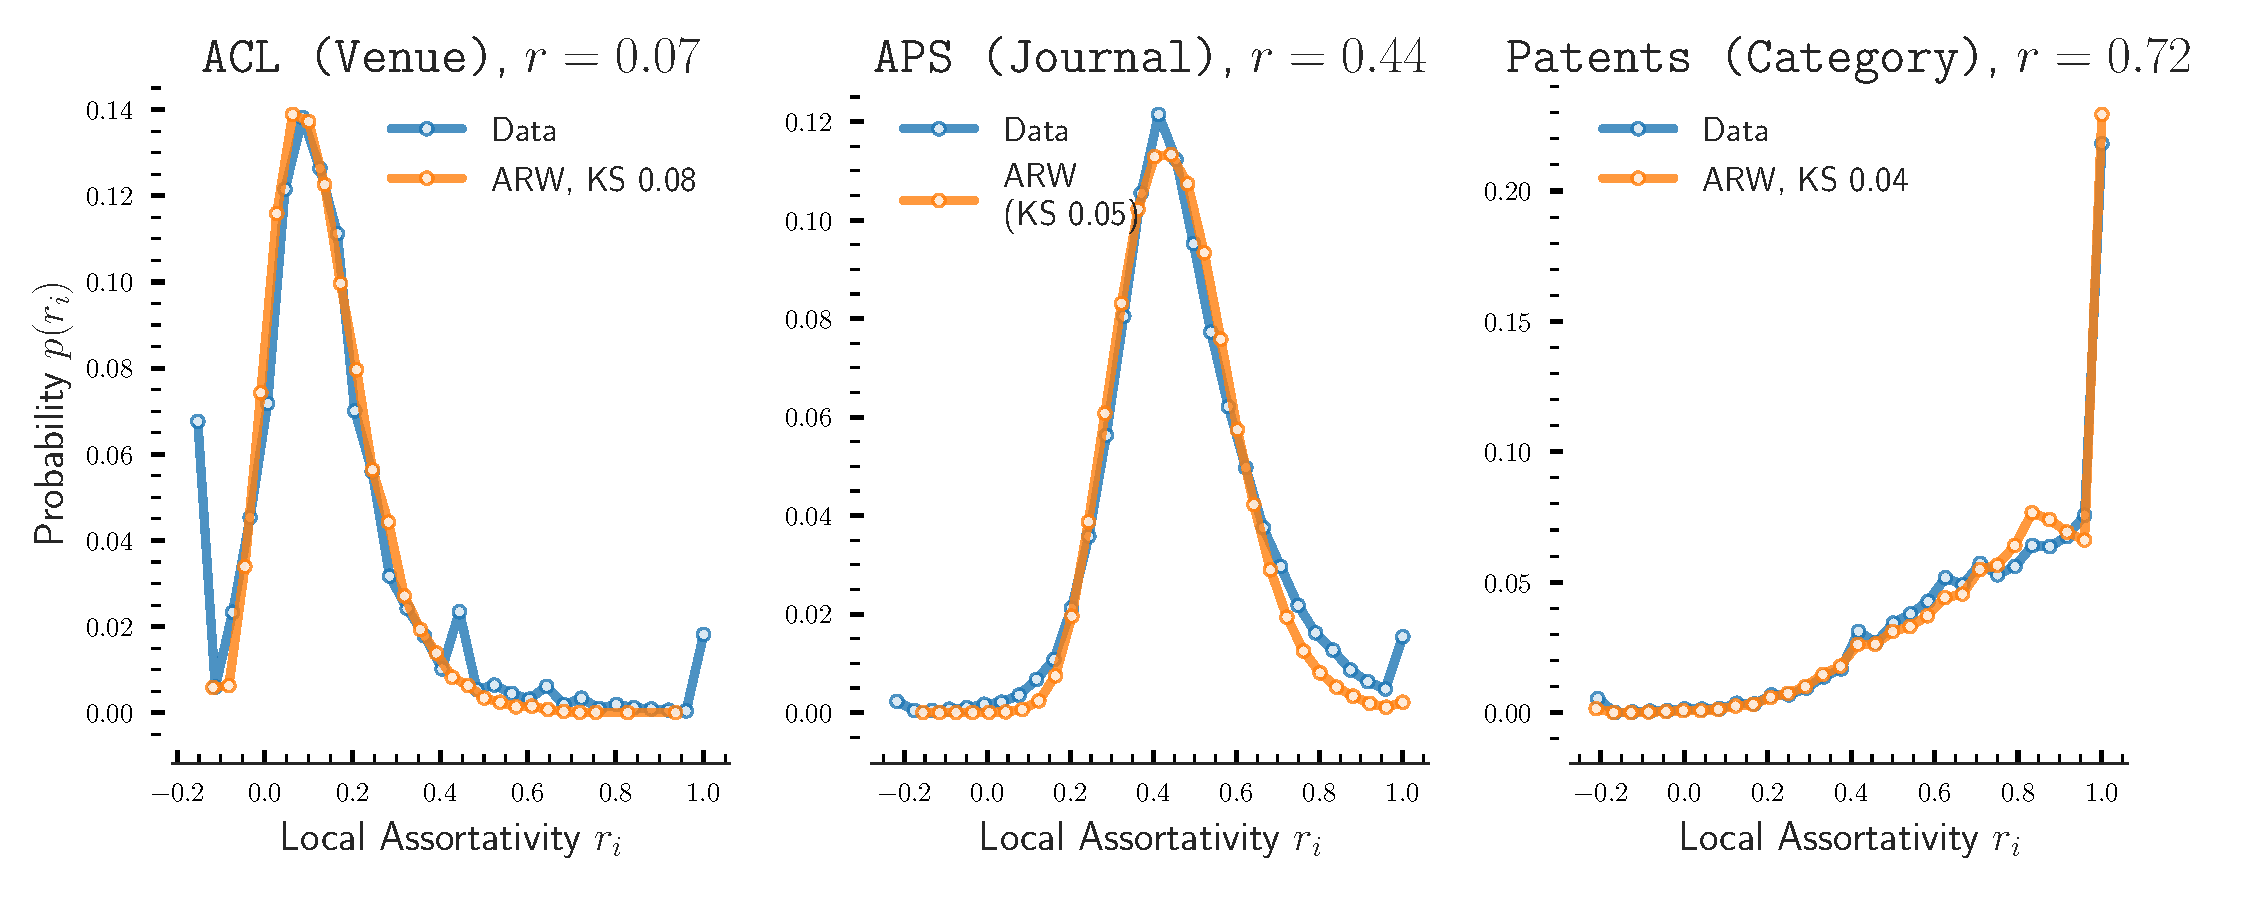
\includegraphics[width=\linewidth]{local_mixing}
	\caption{Local assortativity distributions of attributed networks \texttt{ACL}, \texttt{APS}
		and \texttt{Patents} reveal anomalous, skewed and heterophilic local mixing patterns.
		\texttt{ARW} accurately preserves local assortativity, but does not account for anomalous mixing patterns.}
	\label{fig:local_atty}
	\vspace{-8pt}
\end{figure}
Our model \texttt{ARW} can preserve
diverse local assortativity distributions with high accuracy even though nodes
share the same attribute parameters $\psame$ and $\pdiff$. This is because, in addition
to sampling attributes conditioned on time, \texttt{ARW}
incorporates multiple sources of stochasticity through its edge formation
mechanism. As a result, incoming nodes with fixed homophilic preferences can position
themselves in neighborhoods with variable local assortativity by (a) selecting a seed node in a region
with too few (or too many) similar nodes or (b) exhausting all its links before
visiting similar (or dissimilar) nodes.
We note that \texttt{ARW} is not expressive enough to model anomalous
mixing patterns; richer mechanisms such as sampling $\psame$ or $\pdiff$
from a mixture of Bernoullis are necessary to account for anomalous mixing patterns.
